\chapter{從伊辛磁體到液--氣臨界現象}

\lectureoverview{液--氣轉變可以透過一條出乎意料的途徑來理解。我們先完成伊辛磁體的平均場分析，找出其共存線與臨界點，再將自旋向上重新詮釋為被佔據的晶格位置。由此得到的晶格氣體具有硬核排斥、短程吸引、由磁場控制的化學勢，且相圖完全相同。正式課程以臨界行為與普適性作結。另有一場課後討論，探討物理學家所說的精細調整是什麼、選擇效應如何可能納入解釋，以及為什麼這類推理唯有結合機制與可能的檢驗才有用。}

\section{為什麼要從磁體談起沸水}

沸水是我們想要理解的熟悉現象：液體轉變為氣體，密度也隨之突然改變。標準途徑會經過范德瓦耳斯方程。這裡我們改走另一條路。我們回到伊辛磁體，完成其平均場描述，接著發現同一個模型也可以解讀為流體。

這不只是形象化的類比。正確轉換變數之後，伊辛磁體與晶格氣體就是同一個統計力學系統。磁化強度對應到粒子密度，外加磁場對應到化學勢，磁性共存線則對應到液--氣共存線。這種轉換說明了為什麼兩種表面上不同的物質會具有相同的臨界行為。

平均場在低維系統中無法給出精確的數值答案。在一維中，它甚至預測了精確解所排除的相變。平均場在此的價值在於揭示結構。在二維與三維中，它能找出正確的序參量、彼此競爭的相、臨界端點，以及無窮小偏置如何選定其中一相。在三維中，每個格點有六個最近鄰；以這些近鄰的平均值取代其個別狀態，已足以描繪出有用的定性圖像。

\section{伊辛模型的能量計算}

在超立方晶格的每個格點上放置一個二態自旋，
\begin{equation}
\sigma_i=\pm1.
\end{equation}
我們採用以下哈密頓量：
\begin{equation}
\mathcal H
=-J\sum_{\langle ij\rangle}\sigma_i\sigma_j
+h\sum_i\sigma_i,
\qquad J>0.
\label{eq:ising-hamiltonian}
\end{equation}
記號很重要。第一個總和是對最近鄰\emph{鍵}求和；第二個總和則是對\emph{格點}求和。一條鍵只計算一次，不會從兩個端點各計算一次。

對單一鍵而言，
\begin{equation}
E_{ij}=-J\sigma_i\sigma_j.
\end{equation}
平行自旋的能量為\(-J\)，反平行自旋的能量則為\(+J\)。因此，斷鍵所需的能量為
\begin{equation}
\Delta E_{\rm bond}=+J-(-J)=2J.
\label{eq:broken-bond}
\end{equation}
控制相對玻爾茲曼權重的是數值\(2J\)，而不是任一鍵能量的絕對值。對所有構型加上同一常數，不會改變任何機率。

\begin{classroomqa}
\audiencequestion{為什麼哈密頓量裡有兩種不同的總和？}
\lecturerresponse{交換能屬於一對相鄰格點，因此要對鍵\(\langle ij\rangle\)求和。磁場則獨立作用於每個自旋，因此要對格點\(i\)求和。混淆這兩種計數方式，正好會引入平均場分析中至關重要的因子二。\lecturetimestamp{00:08:04--00:08:45}}
\end{classroomqa}

\begin{classroomqa}
\audiencequestion{增大\(J\)，是否只會讓所有能量都變得更負？}
\lecturerresponse{它會拉大自旋平行與反平行構型之間的能量差。能量零點可以任意選定；有物理意義的是斷鍵需要付出\(2J\)的能量。因此，在溫度固定時，正值\(J\)越大，熱擾動造成的無序就越不利。\lecturetimestamp{00:08:47--00:10:17}}
\end{classroomqa}

在\(d\)維的無限或具週期邊界條件的超立方晶格上，每個格點有\(2d\)個近鄰。若從所有\(N\)個格點逐一計數，每條鍵就會被計算兩次，因此
\begin{equation}
N_{\rm links}=\frac{(2d)N}{2}=dN.
\label{eq:number-links}
\end{equation}
所以，所有自旋排列一致的構型，其交換能為\(-JdN\)。邊界格點會帶來一個表面項；在熱力學極限下，與\(N\)相比可忽略不計。當\(h=0\)時，兩個自旋完全排列一致的狀態簡併。

磁場項確立了一套我們將始終一致採用的符號慣例。在方程~\eqref{eq:ising-hamiltonian}中，正值\(h\)會使\(\sigma=-1\)的格點能量較低。因此，\(h>0\)有利於負磁化強度，而\(h<0\)有利於正磁化強度。若將磁場項改寫為\(-h\sum_i\sigma_i\)，就能反轉這套慣例；物理不會改變，但之後所有符號都必須一併反轉。

\begin{classroomqa}
\audiencequestion{如果哈密頓量只含有\(J\)和\(h\)，溫度是從哪裡進入的？}
\lecturerresponse{溫度透過玻爾茲曼因子\(e^{-\beta\mathcal H}\)進入，其中\(\beta=1/T\)，並採用單位制\(k_{\rm B}=1\)。因此，無因次量是\(\beta J\)和\(\beta h\)。\lecturetimestamp{00:13:07--00:13:43}}
\end{classroomqa}

\section{自旋在近鄰的平均場中}

選取一個遠離邊界的自旋。它有\(2d\)個最近鄰。平均場近似將每個會漲落的近鄰，都以同一個平均值取代：
\begin{equation}
m=\expect{\sigma}.
\end{equation}
涉及所選自旋\(\sigma\)的交換能於是變為
\begin{equation}
-J\sigma\sum_{\text{\(2d\) neighbors}}\sigma_j
\;\longrightarrow\;-2dJm\,\sigma.
\end{equation}
再加上外加磁場，得到單一自旋的有效能量：
\begin{equation}
\mathcal H_{\rm mf}(\sigma)=(-2dJm+h)\sigma.
\label{eq:mean-field-one-spin}
\end{equation}
因子\(2d\)不可或缺。描繪中心自旋的情境時很容易漏掉這個因子；板書推導中曾明確補回。

\begin{figure}[ht]
\centering
\includegraphics[width=0.84\textwidth]{lecture_10_figure_02.png}
\caption{中心自旋被其平均場近鄰包圍的示意圖，並列出單一自旋的能量與逐步導出的自洽方程。}
\lectureframe{00:17:57}
\end{figure}

單一自旋的配分函數為
\begin{align}
z_{\rm mf}
&=\sum_{\sigma=\pm1}
\exp\!\left[-\beta(-2dJm+h)\sigma\right] \\
&=2\cosh\!\left[\beta(2dJm-h)\right].
\end{align}
其平均自旋為
\begin{align}
\expect{\sigma}
&=\frac{\sum_{\sigma=\pm1}\sigma
 e^{\beta(2dJm-h)\sigma}}
{\sum_{\sigma=\pm1}e^{\beta(2dJm-h)\sigma}} \\
&=\tanh\!\left[\beta(2dJm-h)\right].
\end{align}
但所選的自旋應具有代表性，而我們將近鄰的平均值記為\(m\)。因此，自洽條件要求
\begin{equation}
\boxed{m=\tanh\!\left[\beta(2dJm-h)\right].}
\label{eq:mean-field-self-consistency}
\end{equation}
這一個非線性方程，便是將多自旋問題約化為平均場問題的結果。

\begin{classroomqa}
\audiencequestion{為什麼左側的平均值會等於代入每個近鄰的\(m\)？}
\lecturerresponse{這個相等關係正是近似所在。我們假設體相均勻，以平均環境取代實際環境，在此環境中計算中心自旋，再要求算出的平均值重現原先假設的環境。滿足這個條件的解，就是自洽的體相狀態。\lecturetimestamp{00:16:28--00:18:00}}
\end{classroomqa}

引入
\begin{equation}
y=2\beta dJm.
\label{eq:y-definition}
\end{equation}
由於\(\beta=1/T\)，
\begin{equation}
m=\frac{yT}{2dJ},
\end{equation}
方程~\eqref{eq:mean-field-self-consistency}便成為
\begin{equation}
\boxed{\frac{yT}{2dJ}=\tanh(y-\beta h).}
\label{eq:reduced-mean-field}
\end{equation}

\begin{figure}[ht]
\centering
\includegraphics[width=0.82\textwidth]{lecture_10_figure_03.png}
\caption{引入\(y=2\beta dJm\)後的簡化自洽方程，可用圖解法求解。}
\lectureframe{00:24:42}
\end{figure}

\begin{classroomqa}
\audiencequestion{為什麼磁場以\(y-\beta h\)的形式出現？正磁場會偏好哪一種自旋？}
\lecturerresponse{我們的哈密頓量包含\(+h\sigma\)，因此玻爾茲曼指數為\(\beta(2dJm-h)\sigma\)，雙曲正切函數的引數便包含\(y-\beta h\)。正值\(h\)偏好\(\sigma=-1\)。若改以\(-h\sigma\)定義哈密頓量，則\(h\)的每一處都會反號，相圖也會沿水平方向鏡射。\lecturetimestamp{00:18:17--00:20:00}}
\end{classroomqa}

\section{圖解求解與居里點}

令\(h=0\)。我們必須找出下列兩者的交點：
\begin{equation}
\frac{T}{2dJ}y
\qquad\text{and}\qquad
\tanh y.
\end{equation}
第一個是通過原點的直線；第二個是奇函數，且會趨於飽和。在高溫時，直線的斜率較大，唯一交點是\(y=0\)，因此\(m=0\)。溫度下降時，直線的斜率也會變小。直線與雙曲正切曲線在原點相切時，便達到臨界溫度。

\begin{figure}[ht]
\centering
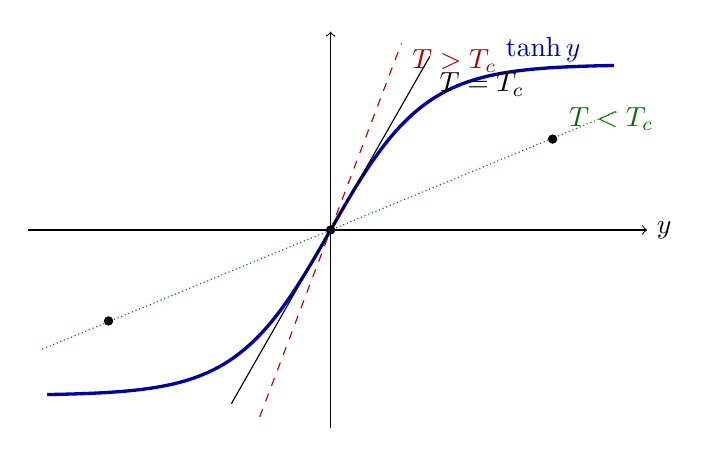
\begin{tikzpicture}[x=1.2cm,y=2.1cm]
\draw[->] (-3.2,0) -- (3.35,0) node[right] {$y$};
\draw[->] (0,-1.2) -- (0,1.2);
\draw[very thick,blue!65!black,domain=-3:3,samples=120]
  plot (\x,{tanh(\x)});
\node[blue!65!black,above] at (2.25,0.96) {$\tanh y$};
\draw[dashed,red!70!black] (-0.75,-1.13) -- (0.75,1.13);
\node[red!70!black,right] at (0.76,1.02) {$T>T_c$};
\draw[black] (-1.05,-1.05) -- (1.05,1.05);
\node[right] at (1.05,0.88) {$T=T_c$};
\draw[densely dotted,green!45!black] (-3.05,-0.72) -- (3.05,0.72);
\node[green!45!black,right] at (2.42,0.67) {$T<T_c$};
\fill (-2.35,-0.55) circle (1.7pt);
\fill (0,0) circle (1.7pt);
\fill (2.35,0.55) circle (1.7pt);
\end{tikzpicture}
\caption{零磁場下的平均場方程。低於\(T_c\)時，兩個非零交點代表穩定的磁化相；零解在代數上仍存在，但已不穩定。}
\label{fig:mean-field-intersections}
\end{figure}

由於
\begin{equation}
\left.\frac{d}{dy}\tanh y\right|_{y=0}=1,
\end{equation}
相切條件為
\begin{equation}
\frac{T_c}{2dJ}=1.
\end{equation}
因此，平均場預測
\begin{equation}
\boxed{T_c^{\rm MF}=2dJ.}
\label{eq:sm10-mean-field-tc}
\end{equation}
低於此溫度時，存在兩個穩定的非零解\(\pm m_0(T)\)。\(m=0\)仍然滿足方程，但已不再是穩定的平衡態。系統會選擇兩個互為對稱的磁化相之一。

\begin{classroomqa}
\audiencequestion{這就是居里溫度嗎？}
\lecturerresponse{是的。對鐵磁體而言，自發磁化消失的溫度通常稱為居里溫度。這裡的\(2dJ\)是平均場給出的居里溫度，不是低維系統的精確結果。\lecturetimestamp{00:28:19--00:28:57}}
\end{classroomqa}

在轉變附近，將雙曲正切函數展開：
\begin{equation}
\tanh y=y-\frac{y^3}{3}+O(y^5).
\end{equation}
在\(h=0\)時，方程~\eqref{eq:reduced-mean-field}給出
\begin{equation}
\left(1-\frac{T}{T_c}\right)y-\frac{y^3}{3}+O(y^5)=0.
\end{equation}
因此，非零分支的行為為
\begin{equation}
y^2\simeq3\left(1-\frac{T}{T_c}\right),
\qquad
m\propto(T_c-T)^{1/2}.
\label{eq:mf-beta-exponent}
\end{equation}
這個平方根律對應一個平均場臨界指數。此指數的精確值在低維系統中不再成立，但序參量在端點連續趨近於零的行為仍會保留。

\section{溫度--磁場平面與分支選擇}

材料決定\(J\)；實驗者則可改變\(T\)和\(h\)。因此，自然會在\(T\)--\(h\)平面上繪製相圖。低於\(T_c\)時，任意微小的磁場都會選定兩個磁化分支之一。依照我們採用的符號慣例，\(h<0\)會選定\(m>0\)，而\(h>0\)會選定\(m<0\)。

在零溫時，自旋完全排列一致，因此\(m=\pm1\)。在高溫時，零磁場下的平均值為\(m=0\)。沿著\(h=0\)趨近臨界點時，磁化強度的絕對值\(m_0(T)\)會連續降至零。但在任一固定的\(T<T_c\)下，穿越\(h=0\)時，磁化強度會從\(+m_0(T)\)不連續地跳到\(-m_0(T)\)。

\begin{figure}[ht]
\centering
\includegraphics[width=0.90\textwidth]{lecture_10_figure_06.png}
\caption{\(T\)--\(h\)平面中的共存線，以及固定溫度低於\(T_c\)時的磁化分支。}
\lectureframe{00:39:30}
\end{figure}

\begin{figure}[ht]
\centering
\resizebox{\linewidth}{!}{%
\begin{tikzpicture}[x=1.25cm,y=1.15cm]
\begin{scope}
\draw[->] (-2.45,0) -- (2.55,0) node[right] {$h$};
\draw[->] (0,0) -- (0,3.7) node[above] {$T$};
\draw[very thick,red!70!black] (0,0) -- (0,2.35);
\fill[red!70!black] (0,2.35) circle (2.3pt);
\node[right] at (0.08,2.35) {$T_c$};
\node at (-1.25,1.05) {$m>0$};
\node at (1.25,1.05) {$m<0$};
\draw[->,rounded corners,blue!65!black] (-1.65,0.85) -- (-1.65,3.02)
 -- (1.65,3.02) -- (1.65,0.85);
\node[blue!65!black] at (0,3.35) {continuous path};
\end{scope}
\begin{scope}[xshift=7.0cm,yshift=1.55cm]
\draw[->] (-2.5,0) -- (2.5,0) node[right] {$h$};
\draw[->] (0,-1.35) -- (0,1.4) node[above] {$m$};
\draw[very thick,blue!65!black]
  (-2.2,1.05) .. controls (-0.75,1.03) and (-0.2,0.75) .. (-0.08,0.62);
\draw[very thick,blue!65!black]
  (0.08,-0.62) .. controls (0.2,-0.75) and (0.75,-1.03) .. (2.2,-1.05);
\draw[dashed] (0,0.62) -- (0,-0.62);
\fill (0,0.62) circle (1.8pt);
\fill (0,-0.62) circle (1.8pt);
\node at (0,-1.75) {\(T<T_c\)};
\end{scope}
\end{tikzpicture}
}
\caption{在固定 \(T<T_c\) 下，磁化強度跨越共存線時會跳變。在完整的雙參數平面中，則可繞過臨界點，連續地連接兩個相。}
\label{fig:ising-phase-plane}
\end{figure}

\begin{classroomqa}
\audiencequestion{如果低於\(T_c\)時磁場恰好為零，會怎麼樣？}
\lecturerresponse{理想的無限系統有兩個同樣穩定的純相。任何與製備過程有關的微小偏置、邊界條件或漲落，都會選定其中一相。在我們採用的符號慣例下，熱力學的不連續性表現在兩個單側極限\(m(T,0^-)=+m_0(T)\)和\(m(T,0^+)=-m_0(T)\)。\lecturetimestamp{00:35:04--00:37:10}}
\end{classroomqa}

\begin{classroomqa}
\audiencequestion{這和遲滯現象是一回事嗎？}
\lecturerresponse{遲滯涉及亞穩態，以及真實系統切換分支時因歷史而延遲的現象。這與此處的討論有關，但需要用到平衡相圖以外的動力學；本節不再探討。\lecturetimestamp{00:37:11--00:37:20}}
\end{classroomqa}

\begin{classroomqa}
\audiencequestion{正相和負相能否在不經歷不連續跳變的情況下連續轉變？}
\lecturerresponse{可以。先將溫度升高至\(T_c\)以上，在該處改變磁場的正負，再降低溫度。這條路徑會繞過端點，磁化強度也會連續變化。只有在固定的\(T<T_c\)下穿越\(h=0\)時，跳變才無法避免。\lecturetimestamp{00:37:20--00:38:15}}
\end{classroomqa}

\begin{classroomqa}
\audiencequestion{\(h\)趨近於零時，磁化強度是否總會趨近於零？}
\lecturerresponse{在低於\(T_c\)的一般溫度下並非如此，此時兩個單側極限都不為零。只有當溫度本身趨近臨界溫度時，自發磁化強度才會趨近於零。\lecturetimestamp{00:38:29--00:39:45}}
\end{classroomqa}

\section{可滲透盒子與化學勢}

現在我們暫且離開磁體，從粒子重新談起。想像一個區域，其勢能低於周圍空間。盒壁可以讓粒子通過，因此粒子能進出盒子。如果盒內能量比盒外低\(\mu\)，粒子佔據盒內相較之下會多出一個玻爾茲曼因子\(e^{\beta\mu}\)。加深或抬高勢阱，會改變盒內粒子的平均數目。

\begin{figure}[ht]
\centering
\includegraphics[width=0.84\textwidth]{lecture_10_figure_07.png}
\caption{可滲透盒子的勢阱示意圖。內外的能量差決定粒子進入盒內的相對偏好。}
\lectureframe{00:41:30}
\end{figure}

\begin{figure}[ht]
\centering
\resizebox{\linewidth}{!}{%
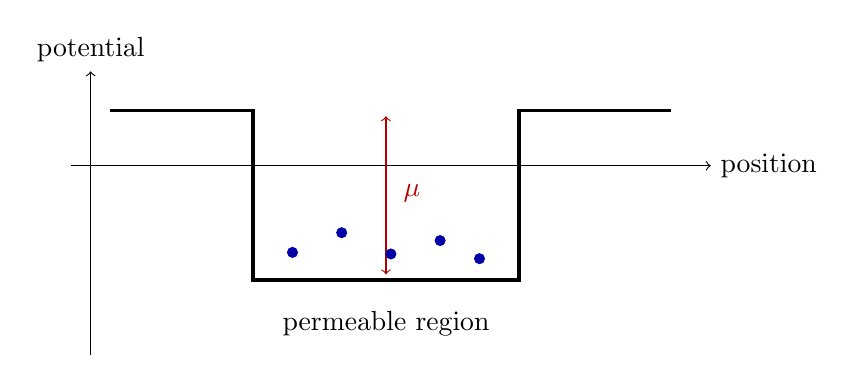
\begin{tikzpicture}[x=1.25cm,y=1.0cm]
\draw[->] (-3.2,0) -- (3.3,0) node[right] {position};
\draw[->] (-3.0,-2.4) -- (-3.0,1.2) node[above] {potential};
\draw[very thick] (-2.8,0.7) -- (-1.35,0.7)
 -- (-1.35,-1.45) -- (1.35,-1.45) -- (1.35,0.7) -- (2.9,0.7);
\draw[<->,red!70!black] (0,0.63) -- (0,-1.38);
\node[right,red!70!black] at (0.08,-0.35) {$\mu$};
\foreach \x/\y in {-0.95/-1.1,-0.45/-0.85,0.05/-1.12,0.55/-0.95,0.95/-1.18}
  \fill[blue!65!black] (\x,\y) circle (2pt);
\node at (0,-2.0) {permeable region};
\end{tikzpicture}
}
\caption{改變位勢的整體偏移，會改變對粒子數的偏好。在巨正則描述中，這個偏移以化學勢表示。}
\end{figure}

這個思想實驗讓化學勢變得具體：相對於粒子庫，每增加一個粒子所獲得的能量優勢。如果有多種粒子都能穿過盒壁，每種粒子便各有其化學勢。密封盒子則不同：此時\(N\)固定，化學勢是由熱力學推得，而不是透過與粒子庫交換粒子來施加。

\begin{classroomqa}
\audiencequestion{勢阱的深度就是化學勢嗎？}
\lecturerresponse{這是直接以力學方式實現化學勢差。將盒內每個單粒子能階降低\(\mu\)，會使能量增加\(-\mu N\)，因此也會使玻爾茲曼指數增加\(+\beta\mu N\)。只有化學勢差具有意義。\lecturetimestamp{00:44:49--00:45:40}}
\end{classroomqa}

由於粒子可以進出盒子，配分和必須納入所有可能的粒子數：
\begin{equation}
\Xi(T,\mu)
=\sum_{N=0}^{\infty}\;\sum_{\mathcal C_N}
\exp\!\left[-\beta E(\mathcal C_N)+\beta\mu N\right].
\label{eq:grand-partition}
\end{equation}
內層總和遍歷粒子數指定為\(N\)時的各種構型；外層總和則遍歷\(N\)本身。巨正則權重也可以寫成\(e^{-\beta(E-\mu N)}\)。

\begin{figure}[ht]
\centering
\includegraphics[width=0.88\textwidth]{lecture_10_figure_08.png}
\caption{可滲透盒子，以及對粒子數與構型所作的巨正則總和。}
\lectureframe{00:47:15}
\end{figure}

\begin{classroomqa}
\audiencequestion{盒子密封後會有什麼改變？}
\lecturerresponse{粒子數不再漲落。此時使用粒子數\(N\)固定的正則配分函數。在可滲透盒子中，\(N\)則是由\(\mu\)控制其平均值的熱力學變數。\lecturetimestamp{00:45:42--00:47:50}}
\end{classroomqa}

在固定溫度下，改變\(\mu\)通常會使密度平滑變化；但低於臨界溫度時，也可能造成密度突然跳變。這正是我們要探討的流體現象。要從微觀層次得到這種現象，粒子必須具備兩個特性：不能彼此佔據同一位置，並且具有短程吸引作用。

\section{將自旋轉換為晶格氣體}

保留晶格，但重新詮釋它的兩種狀態。定義佔據數
\begin{equation}
n_i=\frac{1+\sigma_i}{2}
=
\begin{cases}
0,&\sigma_i=-1,\\
1,&\sigma_i=+1.
\end{cases}
\label{eq:occupation-map}
\end{equation}
空的格點自旋向下；被佔據的格點自旋向上。由於\(n_i\)只能取零或一，因此不允許雙重佔據。晶格本身於是提供硬核排斥。

\begin{figure}[ht]
\centering
\includegraphics[width=0.84\textwidth]{lecture_10_figure_04.png}
\caption{晶格氣體的對應關係從\(\sigma=-1\)代表空格點開始；\(\sigma=+1\)則代表被佔據的格點。}
\lectureframe{00:53:45}
\end{figure}

從空晶格開始，所有格點的自旋都是\(\sigma=-1\)。每條鍵上的自旋都平行，能量為\(-J\)。這個固定的真空能量可以扣除。接著在二維晶格的一個格點上放入一個粒子。對應的自旋翻轉為\(+1\)，使四條鍵斷開。每條斷鍵需要付出\(2J\)的能量，因此
\begin{equation}
\Delta E_1=4(2J)=8J.
\label{eq:one-particle-cost}
\end{equation}
兩個相距甚遠的粒子會使八條鍵斷開，所需能量為\(16J\)。若兩個粒子佔據相鄰格點，它們之間的鍵便重新變為平行。此時只有六條邊界鍵斷開，所需能量為
\begin{equation}
\Delta E_{2,\rm adjacent}=6(2J)=12J.
\end{equation}
因此，將兩個粒子移到一起會使能量降低
\begin{equation}
16J-12J=4J.
\label{eq:lattice-attraction}
\end{equation}
課堂上最初將這項差額說成節省\(2J\)，隨後作了更正：一條共用鍵會消去兩份斷裂邊界鍵的能量，因此吸引能為\(4J\)。

\begin{figure}[ht]
\centering
\includegraphics[width=0.84\textwidth]{lecture_10_figure_05.png}
\caption{二維晶格中的鍵數計算：一個孤立粒子需要\(8J\)，兩個相距甚遠的粒子需要\(16J\)，兩個相鄰粒子則需要\(12J\)。}
\lectureframe{01:00:25}
\end{figure}

晶格氣體現在具備所需的兩種分子性質。二元佔據帶來硬核排斥，交換作用則帶來強度為\(4J\)的最近鄰吸引。自旋翻轉會改變被佔據格點的數目，因此粒子數可以漲落。

\subsection{精確的代數對應關係}

鍵數計算已足以看出物理圖像，但精確的變數轉換能明確顯示兩者等價。將
\begin{equation}
\sigma_i=2n_i-1
\end{equation}
代入方程~\eqref{eq:ising-hamiltonian}。對一條鍵而言，
\begin{equation}
\sigma_i\sigma_j
=4n_in_j-2n_i-2n_j+1.
\end{equation}
在規則的\(d\)維晶格上，
\begin{equation}
\sum_{\langle ij\rangle}(n_i+n_j)=2d\sum_i n_i.
\end{equation}
因此
\begin{align}
\mathcal H
&=-4J\sum_{\langle ij\rangle}n_in_j
+(4dJ+2h)\sum_i n_i+\text{constant}.
\label{eq:ising-as-lattice-gas}
\end{align}
將此式與標準的晶格氣體哈密頓量
\begin{equation}
\mathcal H_{\rm lg}
=-\epsilon\sum_{\langle ij\rangle}n_in_j
-\mu\sum_i n_i+\text{constant}.
\label{eq:lattice-gas-hamiltonian}
\end{equation}
比較，便得到以下對應關係：
\begin{equation}
\boxed{\epsilon=4J,\qquad
\mu=-(4dJ+2h).}
\label{eq:chemical-potential-map}
\end{equation}

\begin{figure}[ht]
\centering
\includegraphics[width=0.88\textwidth]{lecture_10_figure_09.png}
\caption{交換項與磁場項對照粒子能量的計算。磁場會改變粒子的插入能量，卻不改變最近鄰吸引。}
\lectureframe{01:04:30}
\end{figure}

在二維中，插入一個孤立粒子會使能量改變
\begin{equation}
8J+2h=-\mu.
\end{equation}
\(8J\)來自斷鍵；\(2h\)則來自將一個自旋由\(-1\)翻轉為\(+1\)。因此，調整\(h\)會調整化學勢，同時讓吸引作用\(4J\)維持不變。磁場並不直接等於\(\mu\)，因為交換能的基準值帶來了偏移\(4dJ\)。

\begin{classroomqa}
\audiencequestion{如果磁場控制粒子數，為什麼\(h\)不直接就是化學勢？}
\lecturerresponse{相對於空晶格參考態，加入一個粒子也會破壞交換鍵。因此，\(-N\)的標準係數是\(\mu=-(4dJ+2h)\)，而不只是\(-2h\)。這項偏移取決於\(J\)與配位數。\lecturetimestamp{01:06:28--01:06:41}}
\end{classroomqa}

密度的關係同樣簡單：
\begin{equation}
\rho=\expect{n_i}
=\frac{1+\expect{\sigma_i}}{2}
=\frac{1+m}{2}.
\label{eq:density-map}
\end{equation}
因此，\(m=-1\)代表空晶格，\(m=+1\)代表完全填滿的晶格，而\(m=0\)代表半填充。總粒子數為\(N_{\rm p}=\sum_i n_i\)；密度則為\(N_{\rm p}/N\)。

\begin{figure}[ht]
\centering
\includegraphics[width=0.90\textwidth]{lecture_10_figure_10.png}
\caption{密度關係\(\rho=(1+m)/2\)與磁性共存線並列。}
\lectureframe{01:08:25}
\end{figure}

\begin{classroomqa}
\audiencequestion{\((1+m)/2\)代表粒子數還是密度？}
\lecturerresponse{它是每個格點的平均佔據數，因此是無因次的晶格密度。乘上格點總數，便得到預期的粒子總數。區分廣延的粒子總數與強度的密度很重要。\lecturetimestamp{01:06:43--01:09:31}}
\end{classroomqa}

\section{磁性相圖轉化為流體相圖}

根據方程~\eqref{eq:chemical-potential-map}和\eqref{eq:density-map}，重新解讀圖~\ref{fig:ising-phase-plane}。高於\(T_c\)時，改變\(\mu\)會使密度平滑變化。低於\(T_c\)時，越過共存值
\begin{equation}
\mu_{\rm coex}=-4dJ
\qquad(h=0)
\label{eq:coexistence-mu}
\end{equation}
會使密度在稀薄氣體與稠密液體之間跳變。在\(T_c\)時，兩種密度合而為一，不連續性也隨之消失。

\begin{figure}[ht]
\centering
\includegraphics[width=0.92\textwidth]{lecture_10_figure_11.png}
\caption{將伊辛共存線解讀為液--氣相圖。氣體位於低密度側，液體位於高密度側；繞過臨界端點，就能讓兩者連續相接。}
\lectureframe{01:14:30}
\end{figure}

\begin{figure}[ht]
\centering
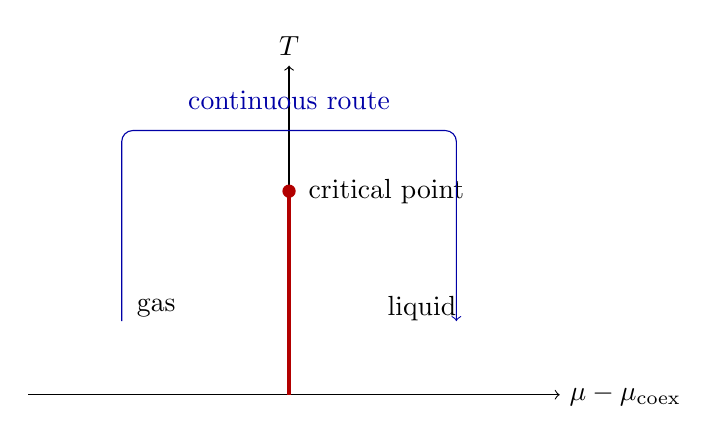
\begin{tikzpicture}[x=1.25cm,y=1.1cm]
\draw[->] (-2.65,0) -- (2.75,0) node[right] {$\mu-\mu_{\rm coex}$};
\draw[->] (0,0) -- (0,3.8) node[above] {$T$};
\draw[very thick,red!70!black] (0,0) -- (0,2.35);
\fill[red!70!black] (0,2.35) circle (2.4pt);
\node[right] at (0.1,2.35) {critical point};
\node at (-1.35,1.0) {gas};
\node at (1.35,1.0) {liquid};
\draw[->,blue!65!black,rounded corners]
 (-1.7,0.85) -- (-1.7,3.05) -- (1.7,3.05) -- (1.7,0.85);
\node[blue!65!black] at (0,3.4) {continuous route};
\end{tikzpicture}
\caption{液體與氣體在端點以下是不同的相，但在超臨界區域，兩者之間沒有奇異邊界。}
\label{fig:liquid-gas-plane}
\end{figure}

這便對應到我們熟悉的沸騰線。在壓力固定時，將液體加熱至越過共存線，就會沸騰。在溫度固定時，改變壓力或化學勢也能越過同一條邊界。過熱蒸氣或過冷液體是超出平衡共存線的亞穩態延續；若要描述它們能維持多久，就需要用到成核動力學，而這不在此處的平衡分析範圍內。

\begin{classroomqa}
\audiencequestion{過熱蒸氣會呈現在這張相圖中嗎？}
\lecturerresponse{平衡相圖標示的是共存邊界。過熱或過飽和狀態屬於亞穩態：由於形成臨界液滴需要付出界面自由能，因此它會暫時停留在平衡邊界的另一側。此處不計算這項動力學修正。\lecturetimestamp{01:12:19--01:12:29}}
\end{classroomqa}

\begin{classroomqa}
\audiencequestion{在一般流體中，如何改變化學勢？}
\lecturerresponse{勢阱盒子是理論上最直接的控制方式。在實驗室中，人們更常改變壓力、體積，或讓系統與粒子庫接觸；熱力學則會將這些控制條件轉換為化學勢的變化。\lecturetimestamp{01:12:30--01:13:59}}
\end{classroomqa}

\begin{classroomqa}
\audiencequestion{密度改變時，分子間勢能\(J\)也會改變嗎？}
\lecturerresponse{不會。對固定的物質而言，\(J\)代表短程吸引作用，在此模型中維持不變。改變\(\mu\)會改變佔據格點的數目，因此也會改變分子間距的分布。改變\(J\)則代表微觀物質或相互作用本身改變。\lecturetimestamp{01:14:50--01:15:41}}
\end{classroomqa}

\begin{classroomqa}
\audiencequestion{臨界溫度就是一般所說的沸點嗎？}
\lecturerresponse{不是。沸點是在指定壓力下決定的，因此壓力改變時，沸點也會沿共存曲線移動。臨界溫度則是唯一的端點；高於此溫度，液體與氣體不再由相邊界分隔。在這個晶格氣體模型中，我們尚未明確推導壓力。\lecturetimestamp{01:15:42--01:17:02}}
\end{classroomqa}

現在可以陳述核心結果。伊辛磁體與晶格氣體不只是相圖相似；經過變數與參數轉換後，兩者具有相同的配分函數。一邊的每一種奇異熱力學性質，在另一邊都有對應：
\begin{equation}
\begin{array}{c|c}
\text{Ising magnet} & \text{lattice gas}\\ \hline
\sigma_i=\pm1 & n_i=0,1\\
m=\expect{\sigma} & \rho=(1+m)/2\\
h & \mu=-(4dJ+2h)\\
\text{aligned exchange} & \text{nearest-neighbor attraction}\\
h=0,\ T<T_c & \text{liquid--gas coexistence}\\
(T_c,0) & \text{critical endpoint}
\end{array}
\label{eq:ising-fluid-dictionary}
\end{equation}

\section{臨界指數與普適性}

在臨界點附近，熱力學量常會呈現冪律奇異行為。以約化溫度
\begin{equation}
t=\frac{T-T_c}{T_c},
\end{equation}
可以概略寫成
\begin{equation}
m\sim(-t)^{\beta_{\rm crit}},
\qquad
\chi\sim |t|^{-\gamma},
\qquad
\xi\sim |t|^{-\nu}.
\label{eq:critical-exponents}
\end{equation}
這裡的\(\beta_{\rm crit}\)是臨界指數，不是反溫度。平均場給出\(\beta_{\rm crit}=1/2\)；但在上臨界維度以下，漲落會改變這些指數。

臨界指數不一定是整數，也不一定全是無理數：二維伊辛模型有幾個著名的精確有理數臨界指數；三維伊辛模型的臨界指數則是非平凡數值，已透過理論與計算以高精度求得。值得把握的重點是，這些指數通常無法單靠初等量綱分析決定。

更令人驚訝的是，微觀細節往往也無法決定這些指數。空間維度相同、序參量對稱性相同，且相互作用具有足夠短程的系統，可能流向相同的長距離臨界理論。它們屬於同一個\emph{普適類}。單軸磁體與一般液--氣系統的臨界端點，都只有一個純量序參量；在相同維度下，兩者屬於伊辛普適類。

\begin{classroomqa}
\audiencequestion{普適類是有限或離散的清單嗎？}
\lecturerresponse{普適類有很多，可依維度、對稱性、守恆律、相互作用範圍及其他長距離特性分類。在許多常見情況下，不動點與臨界指數集合是離散的，但也有臨界指數連續變化的系統。穩妥的說法不是普適類的清單有限，而是許多微觀上不同的系統具有相同的長距離特性。\lecturetimestamp{01:18:50--01:19:38}}
\end{classroomqa}

\begin{classroomqa}
\audiencequestion{液體與氣體共存時，實際容器中是什麼將它們分開？}
\lecturerresponse{是界面。表面張力會抑制界面面積增加；重力則會造成垂直方向的化學勢梯度，通常使密度較高的液體位於氣體下方。若重力可以忽略，界面的形狀便更直接由表面張力與邊界條件決定。\lecturetimestamp{01:19:40--01:21:18}}
\end{classroomqa}

\begin{classroomqa}
\audiencequestion{這幅圖中，汽化熱在哪裡？}
\lecturerresponse{在臨界點以下，跨越一階相共存線通常會伴隨潛熱。接近臨界端點時，兩相逐漸變得相同，因此汽化熱趨近於零。本講建立了相結構，但沒有計算潛熱。 \lecturetimestamp{01:21:19--01:22:18}}
\end{classroomqa}

\begin{classroomqa}
\audiencequestion{相變能否用來製作靈敏的偵測器，例如超導裝置？}
\lecturerresponse{可以。接近相變時，微小擾動可能引發很大的響應，或觸發狀態改變。實際的偵測器會利用這種靈敏度，儘管其中相關的序參量和動力學可能與伊辛模型的例子不同。 \lecturetimestamp{01:22:19--01:24:05}}
\end{classroomqa}

統計力學課程到此結束。課程從熵與平衡談起，經過配分函數與氣體，最後指出磁體與流體可以是同一種臨界現象的兩種描述。

\section{課後討論：精細調節與選擇}

正式講課結束後，談話又持續了約四十分鐘。這段內容值得保留，但不應與上文的推導混為一談。討論主題已不再是格點氣體，而是精細調節的邏輯，以及在宇宙學中謹慎運用人擇選擇的方式。

\subsection{數值小不代表必然經過精細調節}

「\emph{人擇原理}」一詞的各種用法，沒有一句話能一概而論。較實用的出發點是從操作層面來看：若一個理論容許許多實際實現的環境，那麼觀測就必須以觀察者只能在其中某些環境中出現這項事實為條件。這種條件式陳述可以是合理的；但若援引時沒有明確的系綜、選擇條件，或使各種可能性具有物理意義的機制，這種說法就會流於空洞。

在引入選擇效應之前，必須先區分小參數與經過精細調節的參數。某個數值可能很小，是因為穩定的動力學機制會將它驅動至某個特殊值。所謂精細調節，則是指觀測值似乎必須仰賴原本彼此獨立的貢獻之間極其精確的平衡，而且目前沒有已知的復原機制或對稱性來保護這種平衡。

\begin{classroomqa}
\audiencequestion{人擇原理能否明確表述？}
\lecturerresponse{合理的用法是條件式的，而非玄妙的：如果許多實際實現的物理環境具有不同參數，那麼像我們這樣的存在者所觀測到的環境，便是從適合觀察者存在的子集中抽取而來。這個原理本身不會產生這些環境，也不會為它們指定機率；這些工作屬於底層物理學。 \lecturetimestamp{01:25:45--01:26:13}}
\end{classroomqa}

宇宙學常數是引出這項議題的典型例子。與量子場論對真空能所作的粗略估計相比，它的觀測值小得驚人。困難不只是最終數值很小，而是許多大項似乎必須以極高的精度彼此抵銷，同時又沒有公認的低能回饋機制能將結果調整至觀測值。

\subsection{飛艇與潛艇}

兩個浮力例子可以清楚呈現這項差異。飛艇會漂浮在平均密度與周圍空氣密度相等的高度。空氣密度隨高度增加而降低。飛艇上升時，周圍空氣變得更稀薄，飛艇便趨於下降；飛艇下降時，周圍空氣變得更稠密，飛艇便趨於上升。密度相等的數值條件或許微妙，但大氣密度梯度提供了復原回饋，因此這個平衡有動力學機制可解釋。

在近乎不可壓縮的水中，具有中性浮力的潛艇則是另一回事。水的密度隨深度變化很小。如果潛艇的平均密度恰好等於周圍水的密度，就沒有類似的深度依賴復原機制可以解釋兩者為何相等。只要有極小的密度差，潛艇就會上升或下沉。要達到中性浮力，必須精確調整壓艙物與艇內載荷。除非有某種控制系統或設計機制能解釋這項調整，否則這個微小的差值便是精細調節的結果。

\begin{figure}[ht]
\centering
\resizebox{\linewidth}{!}{%
\begin{tikzpicture}[>=Latex]
\begin{scope}[xshift=-3.8cm]
\shade[top color=blue!5,bottom color=blue!28] (-2.5,-2.2) rectangle (2.5,2.2);
\draw[very thick,rounded corners=18pt,fill=yellow!35]
  (-1.15,0) ellipse (1.15 and 0.55);
\draw[thick] (0,-0.55) -- (0,-1.05);
\draw[thick,fill=gray!20] (-0.45,-1.05) rectangle (0.45,-1.38);
\draw[->,red!70!black,thick] (1.65,1.45) -- (1.65,0.55)
 node[midway,right] {restoring};
\draw[->,red!70!black,thick] (-1.65,-1.45) -- (-1.65,-0.55)
 node[midway,left] {restoring};
\node at (0,2.55) {\textbf{Blimp: density gradient}};
\node[align=center] at (0,-2.75) {displacement changes\\the buoyant imbalance};
\end{scope}
\begin{scope}[xshift=3.8cm]
\shade[top color=cyan!10,bottom color=blue!45] (-2.5,-2.2) rectangle (2.5,2.2);
\draw[very thick,fill=gray!35,rounded corners=12pt]
  (-1.45,-0.25) -- (1.1,-0.25) arc (-90:90:0.38)
  -- (-1.45,0.51) -- cycle;
\draw[thick] (-0.25,0.51) -- (-0.25,0.85) -- (0.35,0.85) -- (0.35,0.51);
\draw[->,red!70!black,thick] (1.65,0.15) -- (1.65,1.35)
 node[midway,right] {rise};
\draw[->,red!70!black,thick] (-1.65,0.15) -- (-1.65,-1.35)
 node[midway,left] {sink};
\node at (0,2.55) {\textbf{Submarine: nearly uniform density}};
\node[align=center] at (0,-2.75) {no depth-dependent feedback\\protects neutral buoyancy};
\end{scope}
\end{tikzpicture}
}
\caption{微小的差值可能源自動力學穩定機制，也可能確實經過精細調節。飛艇具有復原回饋；理想化的潛艇則必須調整平均密度，使其與水的密度相等。}
\label{fig:blimp-submarine}
\end{figure}

\begin{classroomqa}
\audiencequestion{既然觀察到中性浮力，為什麼潛艇上的人還要追問原因？}
\lecturerresponse{因為若沒有壓艙控制機制，就沒有對稱性或環境回饋能維持兩個獨立密度相等。問題不在於這種相等在邏輯上是否可能，而在於系統為什麼會落在參數空間中如此狹窄的區域。 \lecturetimestamp{01:35:05--01:36:25}}
\end{classroomqa}

\subsection{多重區域與條件式觀測}

現在設想某個過程產生數量極多、平均密度各不相同的潛艇。大多數潛艇會下沉或上浮，只有極少數能在海面與海底之間適宜生存的區域停留很長時間。必然生活在倖存潛艇中的觀察者，測得接近中性浮力時不應感到意外。觀察者能夠存在的條件，決定了哪些觀測會被選中。

這套推理需要兩項要素：
\begin{enumerate}
\item 實際產生多種可能情況的物理過程，而不是只在想像中存在的各種可能性；
\item 說明觀測為何只會在有限子集中進行的選擇條件。
\end{enumerate}
選擇效應不會取代產生這些情況的機制。系綜一旦存在，選擇效應改變的是觀察者測得某種結果的條件機率。

\begin{classroomqa}
\audiencequestion{這個論證是否只是在說：樣本足夠大時，不太可能發生的事情總會在某處發生？}
\lecturerresponse{這只是論證的前半。後半是觀測條件化：觀察者並非從所有區域中均勻抽樣，而只來自能容許他們存在的區域。完整的主張仍須提出區域的測度，並說明產生這些區域的物理機制。 \lecturetimestamp{01:39:19--01:40:36}}
\end{classroomqa}

套用到真空能上，宇宙學常數若有很大的負值，宇宙可能會過快地重新塌縮；若有足夠大的正值，物質則可能無法凝聚成星系。觀測值落在一個與長壽命結構相容的狹窄範圍內。這可以作為一種可能的選擇條件，但不能據此推導出宇宙學常數的分布。

量子場論帶來了精細調節問題：不同場與不同尺度的真空貢獻，各自都遠大於觀測到的剩餘值。若這些項幾乎完全抵銷，情況就像經過仔細平衡的潛艇，而不像能自我校正的飛艇。這個類比是要揭示其中的邏輯問題，並未提供解答。

\begin{classroomqa}
\audiencequestion{一個參數的變化，能否由其他幾個參數的變化加以補償？}
\lecturerresponse{可以。可行區域未必是某一個參數軸上的狹窄區間，也可能是多維參數空間中的薄曲面。相關聯的變化可以維持結構；但接著就要問，為什麼實際實現的參數會落在該曲面附近，以及底層理論賦予這些參數何種測度。 \lecturetimestamp{01:45:10--01:46:19}}
\end{classroomqa}

\begin{figure}[ht]
\centering
\begin{tikzpicture}[x=1.3cm,y=1.05cm,>=Latex]
\draw[->] (-3.2,0) -- (3.4,0) node[right] {$\lambda_1$};
\draw[->] (0,-2.5) -- (0,2.65) node[above] {$\lambda_2$};
\fill[gray!12] (-3,-2.25) rectangle (3.1,2.3);
\draw[very thick,blue!65!black]
 (-2.8,-1.55) .. controls (-1.3,-0.75) and (0.15,0.05) .. (2.85,1.55);
\draw[very thick,blue!25]
 (-2.8,-1.25) .. controls (-1.3,-0.45) and (0.15,0.35) .. (2.85,1.85);
\fill[blue!15,opacity=.65]
 (-2.8,-1.55) .. controls (-1.3,-0.75) and (0.15,0.05) .. (2.85,1.55)
 -- (2.85,1.85) .. controls (0.15,0.35) and (-1.3,-0.45) .. (-2.8,-1.25) -- cycle;
\node[blue!65!black,rotate=28] at (1.3,0.95) {viable band};
\foreach \x/\y in {-2.4/1.45,-1.7/-1.8,-0.9/1.8,0.3/-1.45,1.2/1.85,2.4/-0.8}
  \fill[red!65!black] (\x,\y) circle (2pt);
\fill[green!45!black] (0.55,0.58) circle (2.8pt);
\node[green!35!black,right] at (0.65,0.55) {observed domain};
\end{tikzpicture}
\caption{若有多個參數，可居住性或結構可行性所占的區域，可能是狹窄而彼此相關的帶狀區域，而非單一參數的狹窄區間。選擇效應會將觀測限制在該區域內，卻不會產生參數分布。}
\label{fig:viable-parameter-band}
\end{figure}

\subsection{景觀假說及其不確定性}

一種可能的替代方案來源，是具有許多亞穩真空的理論；這些真空可能在不同宇宙區域中實現。弦論景觀構想與永恆暴脹情境都是例子，但其具體實現方式與機率測度仍不確定。本講將此視為一種可能性，而非已確立的事實。

如果對稱性能迫使宇宙學常數恰好為零，那會是較傳統的解釋。困難在於，觀測到的加速膨脹對應的是一個小而非零的值。能自然給出零值的機制，不會自動解釋這個微小的剩餘值；對稱性破缺也可能只是重新引入精細調節問題。這裡再次用到潛艇的比喻：一條繩索可以把潛艇固定在選定的深度，但繩索本身就是必須找出來的機制，不能只是假定它存在。

\begin{classroomqa}
\audiencequestion{非常精確地測量某個參數，會違反不確定性原理嗎？}
\lecturerresponse{不會。不確定性關係適用於特定的不對易可觀測量組合。耦合常數或真空參數可以有明確確定的值，而不必是某個未受控制之可觀測量的正則共軛量。測量精確本身並不構成不確定性原理的悖論。 \lecturetimestamp{01:49:21--01:49:36}}
\end{classroomqa}

\begin{classroomqa}
\audiencequestion{人擇推理究竟解釋了這個數值，還是只重述觀察者必須具備這個條件？}
\lecturerresponse{選擇效應本身不是動力學解釋。它的合理用途，是在實際實現的物理系綜中改變條件機率。若沒有系綜、測度或可檢驗的後果，這種說法就可能淪為標籤，而非解釋。 \lecturetimestamp{01:49:37--01:50:21}}
\end{classroomqa}

\subsection{粒子物理中的中等程度巧合}

並非所有與生命相關的參數都經過同等程度的精細調節。普通物質仰賴光子、電子、輕夸克與強作用力；中微子會影響宇宙學，但不是直接束縛原子的媒介。質子--中子質量差的影響尤其重大。由於中子略重於質子，孤立中子會衰變，而普通氫則是穩定的。若兩者質量的大小關係充分反轉，核化學就會發生根本性的改變。

電子質量與精細結構常數也決定了原子的尺度與束縛能。大幅改變它們會改變化學性質。這些敏感度確實值得討論，但不應誇大成「任何微小變化都會排除所有可想像的複雜形式」。與宇宙學常數問題相比，許多這類巧合的程度較為有限，而且與其他參數彼此相關。

與電弱尺度相關的階層問題，是另一個重要的自然性問題：輻射修正往往會使基本純量場的質量對高能尺度十分敏感，除非有額外結構加以保護。它的地位與詮釋都不同於真空能問題，兩者都不應被簡化成一句口號。

\begin{classroomqa}
\audiencequestion{改變質子--中子質量差，真的會影響普通物質嗎？}
\lecturerresponse{會。質量大小關係如同觀測所見，才能容許穩定氫存在，也會影響原子核的貝他穩定性。適度的改變可能重新安排核種豐度與恆星燃燒。仔細分析時，必須一致地改變彼此耦合的參數，而不能只改變一個數值，卻把其他參數全都固定不動。 \lecturetimestamp{01:51:47--01:53:08}}
\end{classroomqa}

\begin{classroomqa}
\audiencequestion{電子質量與精細結構常數分別有什麼作用？}
\lecturerresponse{它們決定原子特徵能量尺度與長度尺度；在單位 \(\hbar=c=1\) 下，示意而言分別為 \(E_{\rm atom}\sim \alpha^2m_e\) 與 \(a_0\sim(\alpha m_e)^{-1}\)。大幅改變它們會重塑化學性質，不過確切的可行區域涉及多個維度。\lecturetimestamp{01:53:09--01:54:12}}
\end{classroomqa}

\subsection{歧見、時間變化與檢驗}

討論短暫轉向對暴脹的批評，以及如何詮釋精密宇宙學資料。對這段歷史上的歧見，應如實呈現其歧見，而非靠修辭強行定論。暴脹有成功的現象學預測，也有許多模型變體；初始條件、測度與可檢驗性等問題仍在討論中。資料能約束模型，但對話中提到某項實驗，並不足以定論整個理論架構。

\begin{classroomqa}
\audiencequestion{宇宙學常數能否緩慢地隨時間變化，而非保持不變？}
\lecturerresponse{動力學暗能量場可以造成隨時間變化的加速膨脹。但這會引入一個位能與初始條件，而它們本身也必須得到解釋；觀測則將狀態方程約束在接近宇宙學常數的範圍。在本講所處時期的討論中，沒有證據要求存在顯著的時間變化。 \lecturetimestamp{01:57:17--01:59:19}}
\end{classroomqa}

\begin{classroomqa}
\audiencequestion{人擇選擇效應本身會生成不同的宇宙或區域嗎？}
\lecturerresponse{不會。選擇效應指出哪些已實現的區域能容納觀察者，但不會創造這些區域。必須另有一種宇宙學機制產生它們，例如暴脹歷程中的真空躍遷。 \lecturetimestamp{01:59:20--01:59:42}}
\end{classroomqa}

因果順序必須保持清楚：
\begin{equation}
\begin{gathered}
\text{laws and initial conditions}\\[-0.15em]
\downarrow\\[-0.15em]
\text{physical environments}\\[-0.15em]
\downarrow\\[-0.15em]
\text{observers and observations}
\end{gathered}
\end{equation}
觀察者不會回頭支配物理定律。只有當我們詢問從已實現環境中抽取的觀察者可能測得什麼時，條件化才會發揮作用。

因此，科學問題不在於這套說法聽起來是否帶有哲學、政治或宗教色彩，而在於該主張是否界定了物理系綜、提出可計算或至少受約束的測度，並帶來能區分不同方案的後果。多真空宇宙學曾討論的可能訊號，包括氣泡區域彼此碰撞留下的痕跡。這類訊號很難作出穩健的預測；在本講所處時期的討論中，也尚未在宇宙微波背景中確立任何此類訊號。缺乏容易進行的檢驗是一項嚴重限制，但不能因此宣稱這個構想為真，也不能據此否定其背後的精細調節問題。

\begin{classroomqa}
\audiencequestion{要具備什麼條件，這套選擇論證才能成為科學理論？}
\lecturerresponse{這項主張需要一種產生各種可能情況的機制、一個機率測度或受控的替代方法，以及可觀測的後果。氣泡碰撞訊號是一種可能的檢驗途徑；但訊號的缺失或模糊，也顯示可檢驗性問題相當棘手。 \lecturetimestamp{02:02:31--02:04:12}}
\end{classroomqa}

課後討論以這種審慎的態度作結。精細調節可能表明某種解釋尚付闕如。對稱性、動力學調整與環境選擇，是邏輯上彼此不同的候選解釋。選擇效應可以是合理解釋的一部分，但必須坦白交代其假設與限制，並將它納入完整的物理解釋之中。
